%%%% Paramétrage du TD %%%%
\def\xxactivite{ \ifprof \normalsize{TD 5 -- Corrigé } \else  \ifcolle Colle \else TD 5\fi \fi} % \normalsize \vspace{-.4cm}
\def\xxauteur{\textsl{Xavier Pessoles}}

\def\xxnumchapitre{Chapitre 2 \vspace{.2cm}}
\def\xxchapitre{\hspace{.12cm} Hyperstatisme}



\def\xxcompetences{%
\vspace{-.5cm}
\footnotesize{
\textsl{%
\textbf{Savoirs et compétences :}\\
\vspace{-.2cm}
\begin{itemize}[label=\ding{112},font=\color{ocre}] 
%\item \textit{Mod2.C34} : chaînes de solides;
\item \textit{Mod2.C34} : degré de mobilité du modèle;
\item \textit{Mod2.C34} : degré d’hyperstatisme du modèle;
\item \textit{Mod2.C34.SF1} : déterminer les conditions géométriques associées à l’hyperstatisme;
\item \textit{Mod2.C34} : résoudre le système associé à la fermeture cinématique et en déduire le degré de mobilité et d’hyperstatisme.
\end{itemize}}}}

\def\xxtitreexo{Système d'inspection pour tubes de guidage}
\def\xxsourceexo{\hspace{.2cm} \footnotesize{Banque PT -- SIA 2009}}

\def\xxfigures{
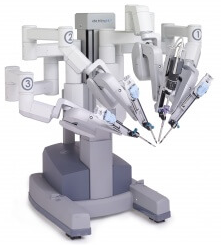
\includegraphics[width=.75\textwidth]{fig_00}
}%figues de la page de garde


\input{\repRel/Style/pagegarde_TD}
\setlength{\columnseprule}{.1pt}

\pagestyle{fancy}
\thispagestyle{plain}

\ifprof
\vspace{5cm}
\else
\vspace{5cm}
\fi

\def\columnseprulecolor{\color{ocre}}
\setlength{\columnseprule}{0.4pt} 

%%%%%%%%%%%%%%%%%%%%%%%

\setcounter{exo}{0}



%\ifprof
%\else
\begin{multicols}{2}
%\fi
\section*{Mise en situation}

\setcounter{numques}{0}




\begin{obj}
L'objectif est de valider le choix de conception de la structure mécanique permettant
de transmettre l'énergie mécanique aux volets.
\end{obj}

Les figures suivantes donnent quelques éléments de la solution adoptée par le bureau d'étude. On y
trouve notamment l'extrémité de la perche sur laquelle est fixée à la tête d'accrochage. La liaison démontable est
réalisée par trois griffes pivotantes qui viennent se loger dans une gorge de la pièce insérée dans le corps de
l'outil d'inspection. Le pivotement des griffes est commandé par une tige coulissant dans la perche sur toute sa
longueur puisque la commande pneumatique ou manuelle est effectuée en haut de la perche, hors d'eau.
On souhaite valider deux des critères d'appréciation :
\begin{itemize}
\item critère 1 : la commande par obstacle dans les deux sens (accrochage et décrochage);
\item critère 2 : la durée de l'accrochage.
\end{itemize}

Les notations adoptées sont les suivantes.

La base orthonormée directe liée au solide $i$  est notée $\mathcal{B}_i = \left(\vect{x_i},\vect{y_i},\vect{z_i}\right)$. Le torseur cinématique du mouvement d’un solide $j$ par rapport à un solide $i$
(ou par rapport au référentiel $\mathcal{R}_i$ lié à celui-ci), réduit en $A$, sera noté $\torseurcin{V}{j}{i}$ $=\torseurl{\vecto{j}{i}}{\vectv{A}{j}{i}}{A}$ $=\torseurl{p_{ji} \vect{x}+q_{ji}\vect{y}+r_{ji}\vect{z}}{u_{ji} \vect{x}+v_{ji}\vect{y}+w_{ji}\vect{z}}{A}$.% où $\left(\vect{x},\vect{y},\vect{z}\right)$ est une base orthonormée associée à la liaison $L_k$. 

Le torseur des actions mécaniques exercées par un solide $i$ sur un solide $j$, réduit en $A$ sera noté $\left\{ \torseurstat{F}{i}{j}\right\}$ $=\torseurl{\vectf{i}{j}}{\vectm{A}{i}{j}}{A}$ $=\torseurl{X_{ij}\vect{x}+Y_{ij}\vect{y}+Z_{ij}\vect{z}}{L_{ij} \vect{x}+M_{ij}\vect{y}+N_{ij}\vect{z}}{A}$.% où $\left(\vect{x},\vect{y},\vect{z}\right)$ est une base orthonormée associée à la liaison $L_k$. 

\subsection*{Validation de la transmission du mouvement de commande} 
\subsubsection*{Étude préliminaire d'un modèle simplifié}
On adopte dans un premier temps, un modèle simplifié, pour une seule griffe, défini par le schéma cinématique
donné dans la figure suivante.


\begin{center}
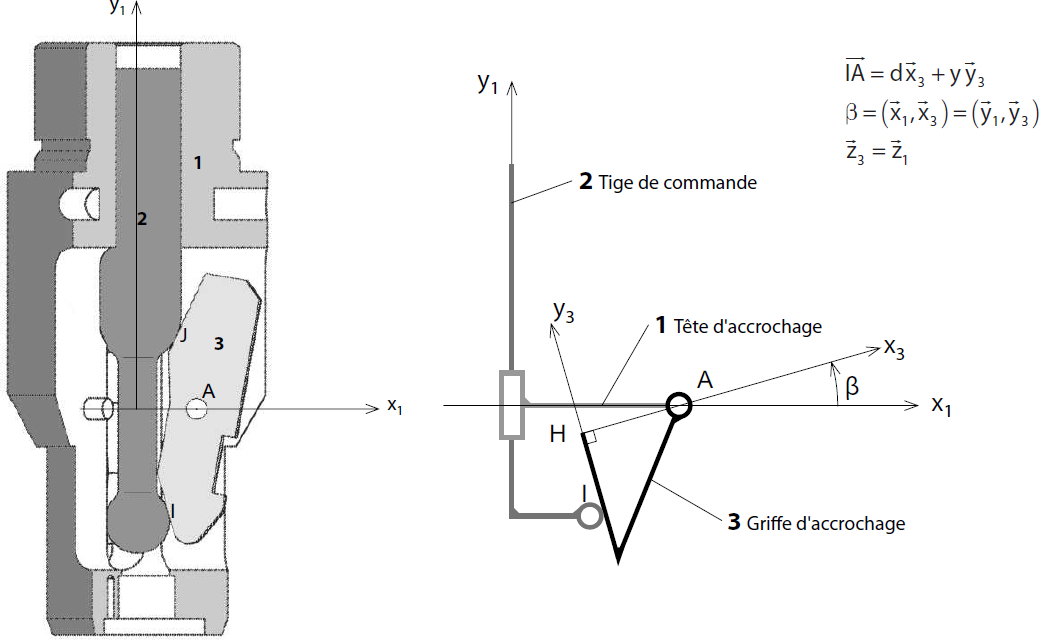
\includegraphics[width=\linewidth]{fig_01}
%\textit{}
\end{center}


\question{En considérant que le modèle est spatial, donner le graphe de structure (graphe des liaisons) associé au schéma cinématique proposé en précisant les éléments géométriques caractéristiques de chaque liaison puis
la forme de leur torseur cinématique $\torseurcin{V}{j}{i}$, c'est-à-dire l'expression des éléments de réduction en fonction des paramètres $p_{ij}$, $q_{ij}$, $r_{ij}$, $u_{ij}$, $v_{ij}$ et $w_{ij}$ dans la base locale de la liaison.}
\ifprof
\begin{corrige}~\\
\end{corrige}
\else
\fi

\question{Établir le système de six équations, en projection dans la base $\mathcal{B}_{3}$ liée au solide 3, traduisant la fermeture cinématique du mécanisme, en fonction des paramètres cinématiques introduits à la question précédente et des paramètres géométriques définis sur la figure précédente.}
\ifprof
\begin{corrige}~\\
\end{corrige}
\else
\fi


\question{Évaluer le rang du système d'équations obtenu et en déduire le degré de mobilité du mécanisme. On supposera
que le paramètre cinématique d'entrée $w_{21}$ est connu et que l'angle $\beta$ est différent de zéro.
Si on fait l'hypothèse que les liaisons sont parfaites, ce modèle est-il hyperstatique ?}
\ifprof
\begin{corrige}~\\
\end{corrige}
\else
\fi

\subsubsection*{Étude du modèle associé à la commande d'une griffe}
Afin d'obtenir une commande par obstacle dans les deux sens de commande, le modèle est complété par une
seconde liaison sphère-plan, telle que le schéma cinématique devienne celui de la figure suivante.

\begin{center}
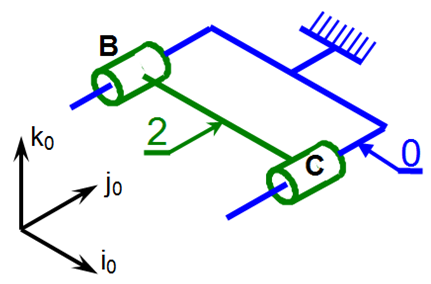
\includegraphics[width=.8\linewidth]{fig_02}
%\textit{}
\end{center}
\begin{obj}
On cherche ici à montrer qu'il est impossible d'obtenir ce double contact avec la géométrie actuelle.
\end{obj}



\question{En vous appuyant sur les résultats précédents et en supposant que les angles $\beta$ et $\beta'$ sont différents de zéro, donner la valeur du degré de mobilité de ce modèle puis son degré d'hyperstatisme. Que concluez-vous de ces résultats ? On notera $\torseurcin{V}{`3}{2}$ le torseur cinématique de la liaison sphère-plan de centre $J$ dont on précisera la normale.}
\ifprof
\begin{corrige}~\\
\end{corrige}
\else
\fi

\question{En supposant que les normales, à préciser, aux liaisons sphère-plan, de centres $I$ et $J$, sont concourantes au point que l'on notera $I_{32}$, déterminer, en utilisant l'équivalence statique, la liaison équivalente entre les solides 3 et 2 au point $I_{32}$.}
\ifprof
\begin{corrige}~\\
\end{corrige}
\else
\fi

\question{Compléter le schéma cinématique avec la liaison équivalente.}
\ifprof
\begin{corrige}~\\
\end{corrige}
\else
\fi
\begin{center}
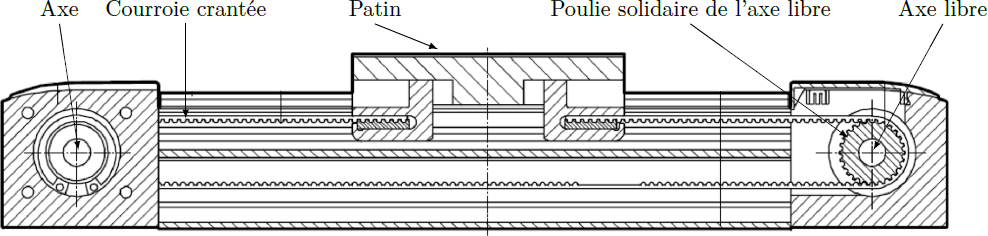
\includegraphics[width=\linewidth]{fig_04}
%\textit{}
\end{center}

\question{Calculer le degré de mobilité du mécanisme ainsi modélisé et comparer cette valeur à celle trouvée à la question \ref{q4}, en supposant les valeurs de $a$ et $b$ quelconques, définies par $\vect{AI}_{32}=a\vect{x_1}+b\vect{y_1}$.}
\ifprof
\begin{corrige}~\\
\end{corrige}
\else
\fi

\question{Indiquer à quelle condition sur a et/ou b, le degré de mobilité serait égal à 1. Commentez ce résultat en regard de l'objectif énoncé plus haut.}
\ifprof
\begin{corrige}~\\
\end{corrige}
\else
\fi

Les valeurs de $a$ et $b$ étant des fonctions du temps, on constate que la condition trouvée ne peut être réalisée
à chaque instant du mouvement d'accrochage, en conservant, sur la pièce 3, deux rampes rectilignes pour les
contacts ponctuels en $I$ et $J$.

Une simulation informatique du mécanisme montre que si on décide de conserver la rampe rectiligne
uniquement au contact en $I$, il est nécessaire d'avoir un profil bombé, donné sur la figure suivante, pour
le contact en $J$.

\begin{center}
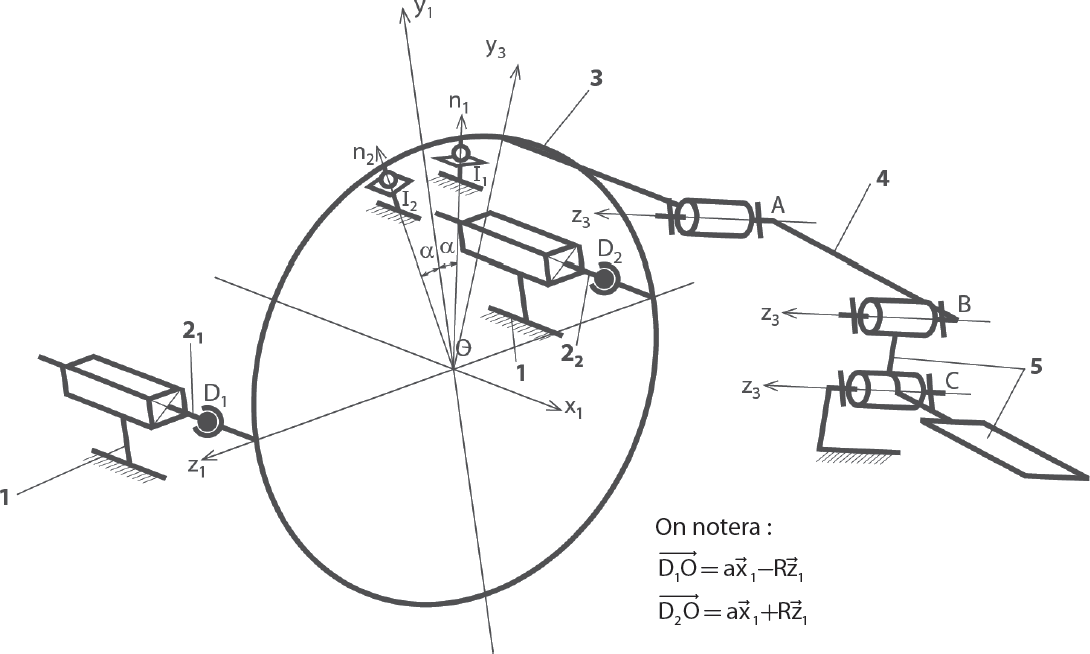
\includegraphics[width=\linewidth]{fig_05}
%\textit{}
\end{center}

\question{Expliquer et effectuer, le tracé permettant de trouver exactement la position du
point de contact $J$, entre la surface sphérique de la tige de commande et le profil bombé de la griffe, obtenu
dans la position représentée.}
\ifprof
\begin{corrige}~\\
\end{corrige}
\else
\fi



\question{Le bureau d'étude a finalement décidé de conserver les deux rampes rectilignes repérées $\Delta I$ et $\Delta J$ sur la figure. Quelle conséquence a ce choix sur le fonctionnement du mécanisme d'accrochage ?
Peut-on valider le critère étudié de la FT 2.1.1 ?}
\ifprof
\begin{corrige}~\\
\end{corrige}
\else
\fi


\subsection*{Validation de la transmission de l'effort de commande}


On souhaite vérifier que le mouvement de commande de la griffe est toujours possible. Pour cela, on se
place dans la configuration du modèle simplifié donné figure 5 de l'Annexe 4. On suppose que seule la liaison
sphère-plan de centre $I$ n'est pas parfaite avec un coefficient de frottement au contact $f$ de 0,2. On suppose
négligeable le poids de la griffe 3 devant les actions mécaniques transmises. On précise que $d=\SI{10}{mm}$ et que
y varie entre 20 et \SI{32}{mm}.

\question{Préciser, en justifiant votre réponse, si un phénomène d'arc-boutement peut se produire au cours du mouvement
de la griffe ? Peut-on valider la solution proposée ?}
\ifprof
\begin{corrige}~\\
\end{corrige}
\else
\fi







\end{multicols}
